% This part is the latex header. It defines what kind of document this will be and 
% says which packages to use. Packages let you include different kind of formats
% and templates in the document. 
\documentclass[11pt]{article} % document type - other options are journal or book?
\usepackage[pdftex]{graphicx} % package to import figures
\usepackage{float} % used for placing figures - H
\usepackage{hyperref} % used for including links (hyper links)
\usepackage{enumerate} % used for making lists
\usepackage[margin=1cm]{geometry}
\usepackage{tabularx}
\usepackage{booktabs}
\usepackage{amsmath}
\usepackage[version=3]{mhchem} 
\usepackage{siunitx}

% math packages
\usepackage{amssymb}
\usepackage{amsmath}

\pagestyle{headings}
\topmargin -0.5in
\oddsidemargin 0.0in
\textwidth 6.5in
\textheight 9.0in

% declare the title, date and author
\title{Radial Bias Pilot 1}
\date{Jan 20, 2021}
\author{Rania Ezzo}

% This is where the actual document starts
\begin{document}
\maketitle
\tableofcontents


\section{Goal of Pilot 1}
To measure radial direction bias with 1D drifting gratings at 2-4 polar angle locations at a given eccentricity. A total of 4 directions of motion will be tested, 2 radial (inwards and outwards) and 2 tangential (clockwise, counterclockwise), to measure the performance differences between (1) centrifugal and centripetal motion directions, and (2) radial and tangential motion directions. 

\subsection{Parameters}
Eccentricity from central fixation: 7 degrees
\\
Locations tested (polar angle relative to fixation): Upper left (45 deg) and lower right (225 deg)
\\
Stimulus: sine wave gratings w/ 0.4 deg sigma gaussian mask
\\
Stimulus spatial frequency: 1 c/deg
\\
Stimulus drift speed: 4 deg/s
\\
Stimulus contrast: full contrast + gaussian mask
\\
Stimulus aperature diameter: 2.5 deg
\\
Black circular aperature was put onto screen to avoid perceptual artifacts from screen edges
\\
Number of subjects: 1

\subsection{Experimental Design}
The pilot uses a 2AFC paradigm, where each trial includes a drifting grating presented at 1 of 2 possible positions, while the subject maintains fixation at the central dot. A method of constant stimuli is used which is set based on the performance of the training session (see Methods). The angular values added to the internal reference frame is chosen at random from the following constants [-1.5, -1.25, -1, -0.75, -0.5, 0.5, 0.75, 1, 1.25, 1.5]. The observer must determine whether the direction of motion if clockwise or counterclockwise relative to the internal reference. The sequence of each trial for the 4 motion standards at one location is depicted below:

\begin{figure}[H]
\centering % centers the figure
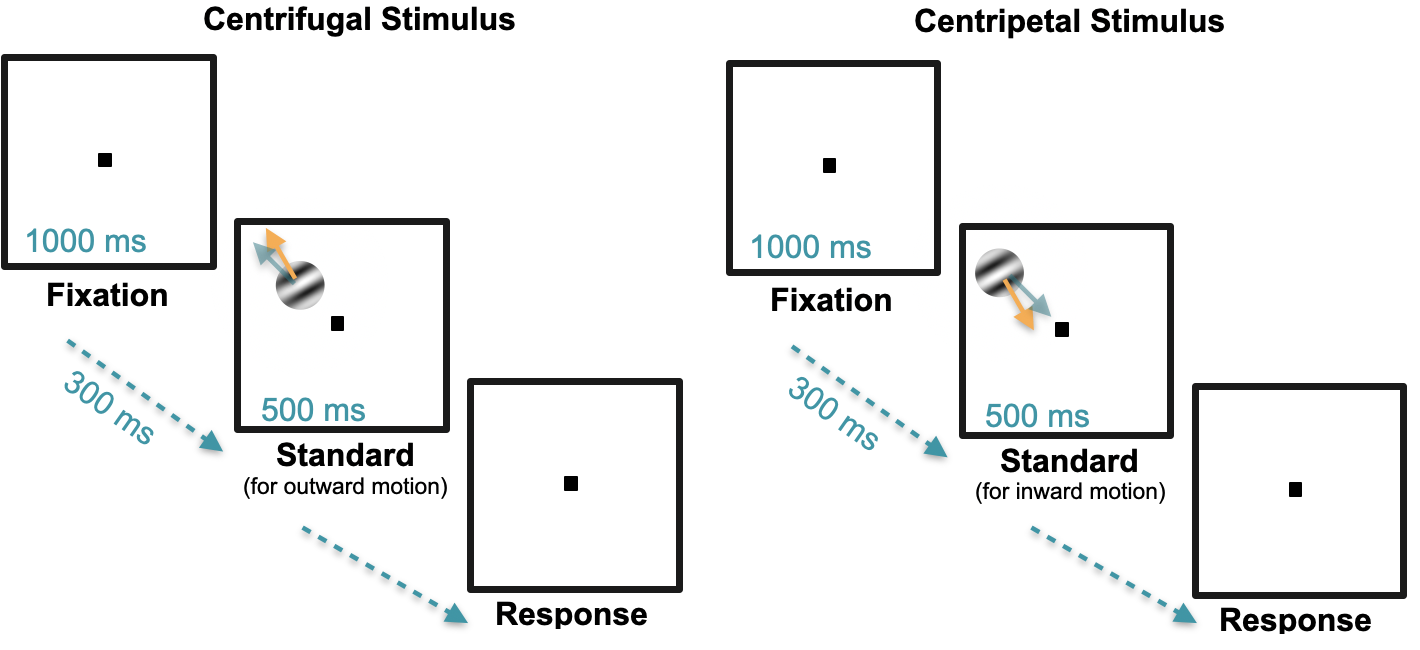
\includegraphics[scale=.4]{Images/Radial_sequence.png}
\\
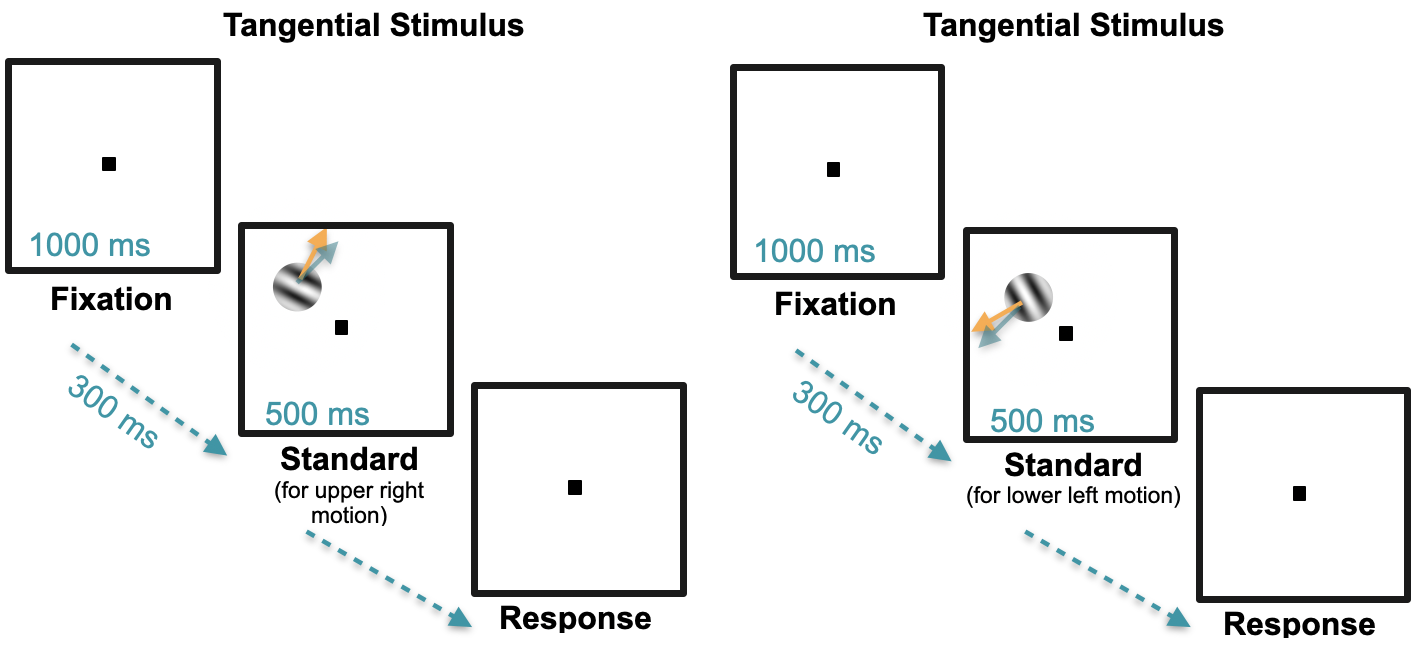
\includegraphics[scale=.4]{Images/Tang_sequence.png}
\caption{Blue arrow represents the internal reference, the orange arrow represents an example of the direction at which the stimulus is presented (can be clockwise or counterclockwise to the blue arrow.}
\end{figure}

\subsection{Block sequence}
Four blocks were run, and each block corresponded to 1 of the 4 conditions being tested (tangential lower left motion, tangential upper right motion, radial upper left motion, radial lower right motion). The internal reference frames for each block is shown below:

\begin{figure}[H]
\centering % centers the figure
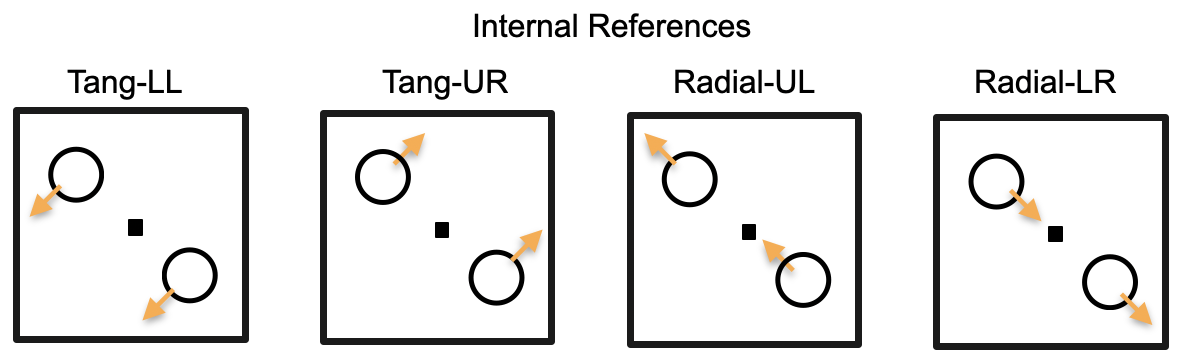
\includegraphics[scale=.4]{Images/Blocks.png}
\end{figure}

Prior to the experiment, the "standard" motion direction corresponding to that specific block is showed to the observer to use as an internal reference. Then a training session is conducted to determine how much tilt is required to meet 75\% accuracy with staircase procedure (MLPest), and to allow subject to practice task with feedback. This was tested using radial motion only, and ~1.5 degrees was the estimated angular value to add/subtract to the standard to achieve 75\% performance of the clockwise/counterclockwise discrimination task. Constants [-1.5, -1.25, -1, -0.75, -0.5, 0.5, 0.75, 1, 1.25, 1.5] were chosen to roughly center around this value for all 4 conditions. Note positive and negative values for clockwise v. counterclockwise tilt.
\\
%Each block contains (2 locations with clockwise/counterclockwise motion) x 80 repetitions = 1,280 trials. All 4 full-blocks took 80 min. 
Each condition (radial-in, radial-out, tang) contained 2 locations x 9 tilt values x 2 (clock v cc) x 20 repetitions = 720 trials. Each full-block takes ~35 min; all 3 full-blocks took 105 min. 
\\
Sequence of partial-blocks tested (re-test was in reverse order): 
\begin{enumerate}
\item radial-UL [angles: +- 0.5, 0.75, 1, 1.25, 1.5] (20 min, 40 trials) - BLOCK1a
\item radial-LR [angles: +- 0.5, 0.75, 1, 1.25, 1.5] (20 min, 40 trials) - BLOCK2a
\item tang-UR [angles: +- 0.5, 0.75, 1, 1.25, 1.5] (10 min, 20 trials) - BLOCK3a
\item tang-LL [angles: +- 0.5, 0.75, 1, 1.25, 1.5] (10 min, 20 trials) - BLOCK3b
\item tang-LL [angles: +- 2, 2.5, 3, 4] (8 min, 20 trials) - BLOCK3c
\item tang-UR [angles: +- 2, 2.5, 3, 4] (8 min, 20 trials) - BLOCK3d
\item radial-LR [angles: +- 2, 2.5, 3, 4] (15 min, 40 trials) - BLOCK2b
\item radial-UL [angles: +- 2, 2.5, 3, 4] (15 min, 40 trials) - BLOCK1b
\end{enumerate}

\section{Data}
\subsection{Psychometric Function (Cumulative normal)}
\begin{figure}[H]
\centering % centers the figure
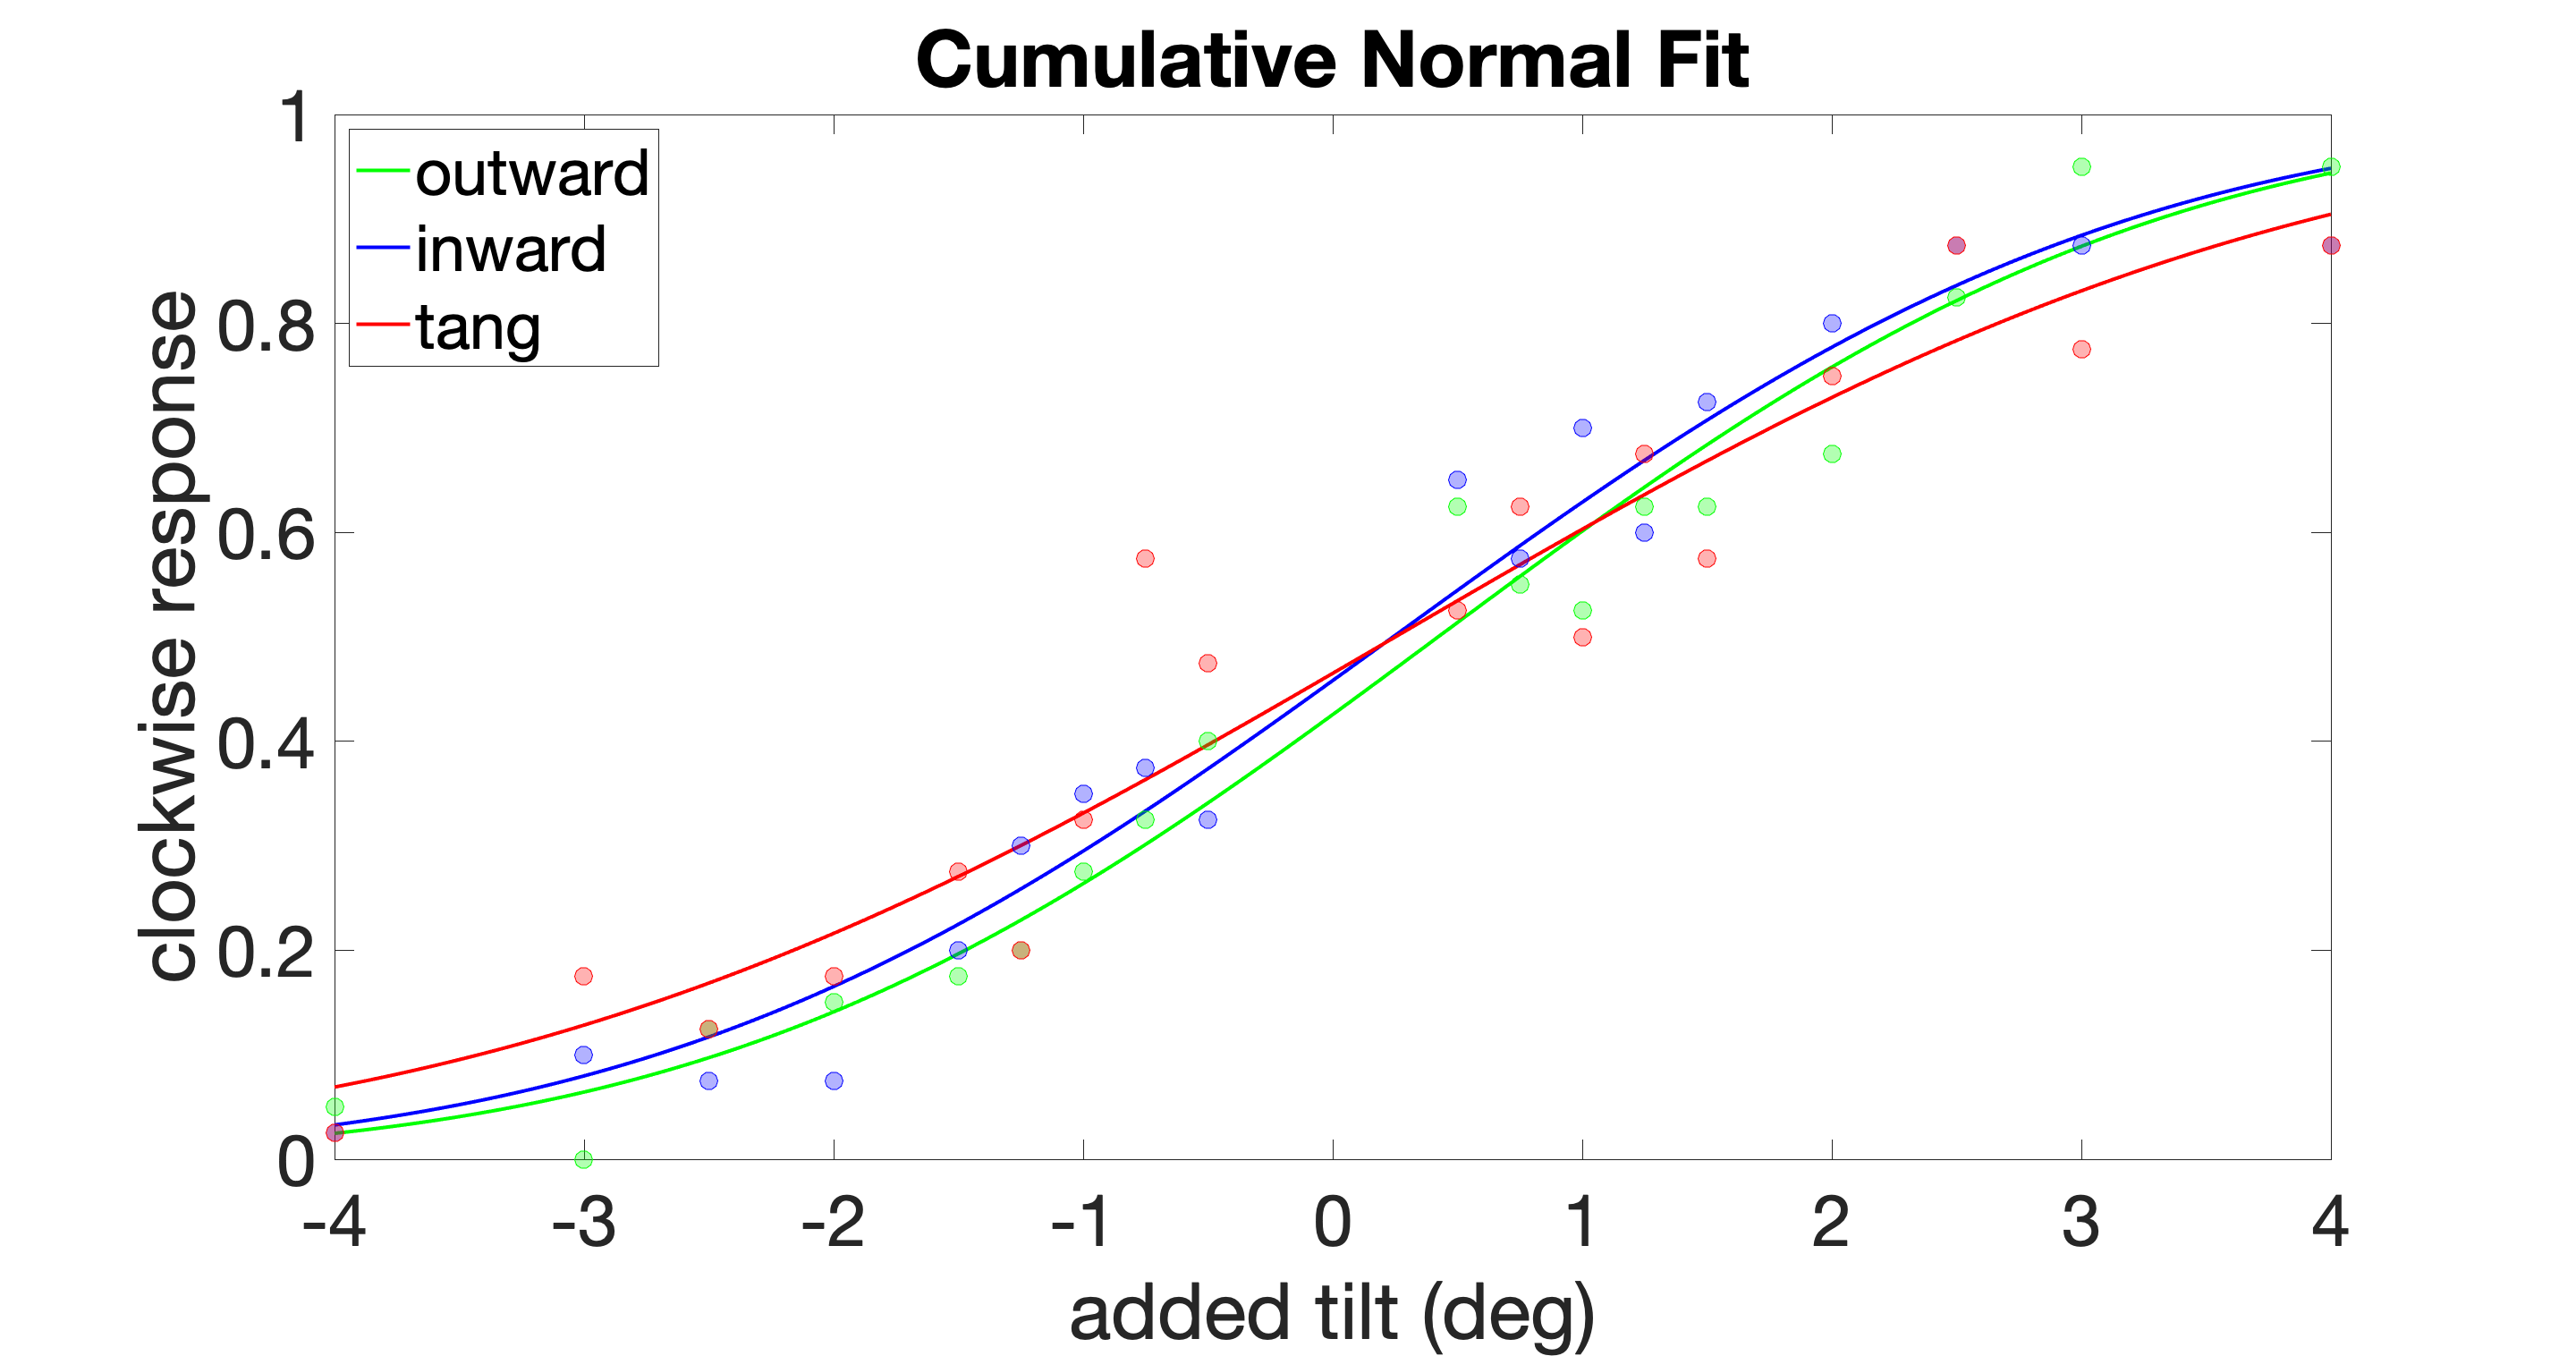
\includegraphics[scale=.08]{Images/PF_set1.png}
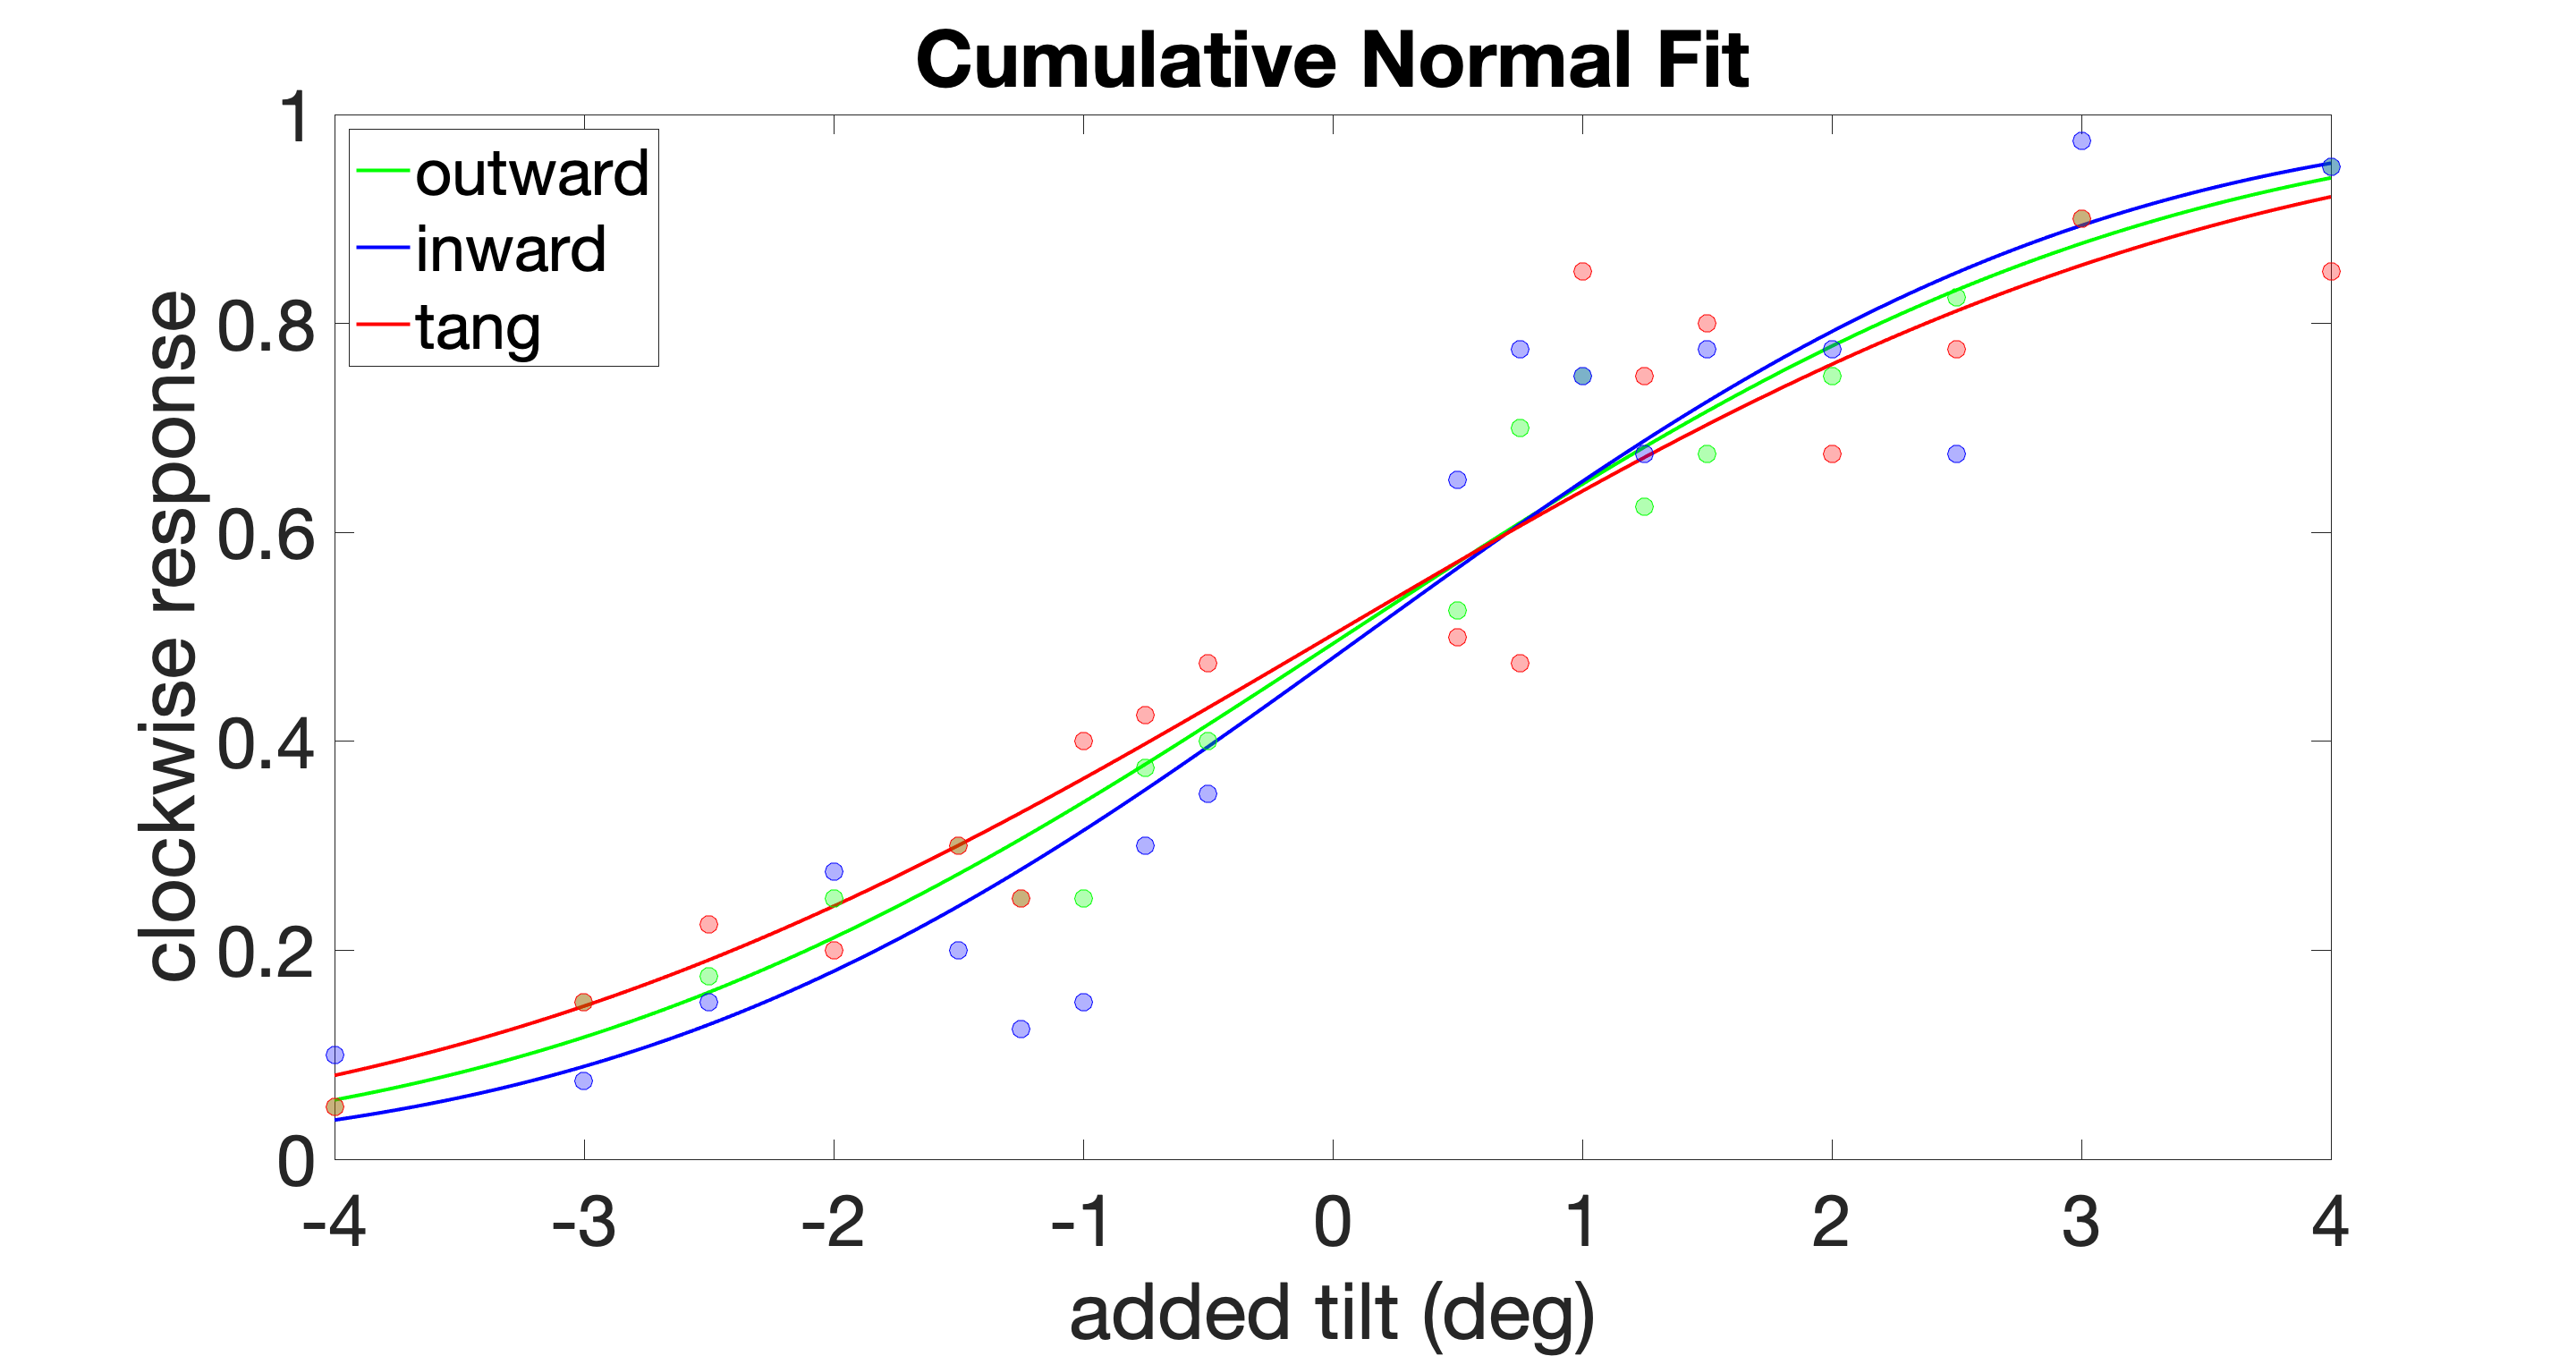
\includegraphics[scale=.08]{Images/PF_set2.png}
\caption{To the left: test data with blocks that contain same reference vector; combines data across locations (40 trials per angle). To the right: re-test with same number of trials.}
\end{figure}

\textbf{SENSITIVIY/SLOPE}
\\
Radial out beta = [test 0.4441], [re-test 0.3914]
\\
Radial in beta = [test 0.4339], [re-test 0.4324]
\\
Tangential beta = [test 0.3488], [re-test 0.3521]
\\
\textbf{BIAS}
\\
Radial out alpha = [test 0.4225]; [re-test 0.0425]
\\
Radial in alpha = [test 0.242]; [re-test 0.1172]
\\
Tangential alpha = [test 0.2512]; [re-test -0.014]

\newpage
\subsection{Current number of trials}
N\_Trials is the total number of trials for a particular condition.
Ans\_clock is the percentage of the observer answering clockwise out of the N\_Trials for that condition.
\begin{table*}[htb]
  \label{tbl:stats-and-correlations}
  %\small\begin{tabularx}{\linewidth}{X*{15}{c}}
  \small\begin{tabular*}{\linewidth}{l@{\extracolsep{\fill}}*{18}{c}}
    \toprule
    & \multicolumn{4}{c}{\textbf{Radial outwards}}\\ \cmidrule(r){2-18}
    & {-4} & {-3} & {-2.5} & {-2} & {-1.5} & {-1.25} & {-1} & {-.75} & {-.5} & {.5} & {.75} & {1} & {1.25} & {1.5} & {2} & {2.5}& {3}& {4} \\ [0.5ex]
    N\_Trials:  &    40 &    40 &    40 &    40 &    40 &    40 &    40&   40 &   40 &    40&    40&    40&   40&    40&    40 & 40 & 40 & 40\\
    Ans\_clock:  &  .05 &  0 &    .13 &    .15 &    .18 &    .2 &    .28 &   .33 &    .4&    .63&    .55&    .53&    .63&    .63&    .68&    .83 & .95 & .95\\
    N\_Trials:  &    40 &    40 &    40 &    40 &    40 &    40 &    40&   40 &   40 &    40&    40&    40&   40&    40&    40 & 40 & 40 & 40\\
    Ans\_clock:  &  .05 &  .15 &    .18 &   .25 &    .3 &    .25 &   .25 &    .38&    .4&    .53&    .7&    .75&    .63&    .68&    .75 & .83 & .9 & .95\\
    \bottomrule
  %\end{tabularx}
  \end{tabular*}
\end{table*}

\begin{table*}[htb]
  \label{tbl:stats-and-correlations}
  %\small\begin{tabularx}{\linewidth}{X*{15}{c}}
  \small\begin{tabular*}{\linewidth}{l@{\extracolsep{\fill}}*{18}{c}}
    \toprule
    & \multicolumn{4}{c}{\textbf{Radial inwards}}\\ \cmidrule(r){2-18}
    & {-4} & {-3} & {-2.5} & {-2} & {-1.5} & {-1.25} & {-1} & {-.75} & {-.5} & {.5} & {.75} & {1} & {1.25} & {1.5} & {2} & {2.5}& {3}& {4} \\ [0.5ex]
    N\_Trials:  &    40 &    40 &    40 &    40 &    40 &    40 &    40&   40 &   40 &    40&    40&    40&   40&    40&    40 & 40 & 40 & 40\\
    Ans\_clock:  &  .03 &  .1 &    .08 &    .08 &    .2 &    .3 &    .35 &   .38 &    .33&    .65&    .58&    .7&    .6&    .73&    .8&    .88& .88 & .88\\
    N\_Trials:  &    40 &    40 &    40 &    40 &    40 &    40 &    40&   40 &   40 &    40&    40&    40&   40&    40&    40 & 40 & 40 & 40\\
    Ans\_clock:  &  .1 &  .08 &    .15 &    .28 &    .2 &    .13 &    .35 &   .15 &    .3&    .35&    .65&    .78&    .75&    .68&    .78&    .78& .68 & .98\\
    \bottomrule
  %\end{tabularx}
  \end{tabular*}
\end{table*}


\begin{table*}[htb]
  \label{tbl:stats-and-correlations}
  %\small\begin{tabularx}{\linewidth}{X*{15}{c}}
  \small\begin{tabular*}{\linewidth}{l@{\extracolsep{\fill}}*{18}{c}}
    \toprule
    & \multicolumn{4}{c}{\textbf{Tangential (combined)}}\\ \cmidrule(r){2-18}
    & {-4} & {-3} & {-2.5} & {-2} & {-1.5} & {-1.25} & {-1} & {-.75} & {-.5} & {.5} & {.75} & {1} & {1.25} & {1.5} & {2} & {2.5}& {3}& {4} \\ [0.5ex]
    N\_Trials:  &    40 &    40 &    40 &  40 &  40 &    40 &    40&   40 &   40 &    40&    40&    40&   40&    40&    40 & 40 & 40 & 40\\
    Ans\_clock:  &  .03 &  .18 &    .13 & .18 &  .28 &    .2 &    .33 &   .58 &    .48&    .53&    .63&    .5&    .68&    .58&    .75&   .88 & .78 & .88\\
    N\_Trials:  &    40 &    40 &    40 &  40 &  40 &    40 &    40&   40 &   40 &    40&    40&    40&   40&    40&    40 & 40 & 40 & 40\\
    Ans\_clock:  &  .05 &  .15 &    .23 & .2 &  .3 &    .25 &    .4 &   .43 &    .48&    .5&    .48&    .85&    .75&    .8&    .68&   .78 & .9 & .85\\
    \bottomrule
  %\end{tabularx}
  \end{tabular*}
\end{table*}


\section{Updates} 
\begin{itemize}
\item Design Related
	\begin{itemize}
	\item Changed blocks to include vectors of the same direction so the subject does not have to change internal reference frame within block
	\item Ran an equal number of trials (sample without replacement).
	\item Left out condition with 0 degrees added tilt (not needed).
	\item Included feedback for all trials to reinforce knowledge of internal stimulus.
	\item Changed stimulus presentation 0.5 sec and fixation period to 1 sec.
	\item Tested with new set of constant stimuli {-4, -3, -2.5, -2, -1.5, -1.25, -1, -0.75, -0.5, 0.5, 0.75, 1, 1.25, 1.5, 2, 2.5, 3, 4}.
	\end{itemize}
\item Analysis Related
	\begin{itemize}
	\item Calculated bias (alpha), and slope for the PFs
	\item Ran experiment 2x (once for each block) to a test-retest validation, and plot.
	\end{itemize}
\item Other improvements
	\begin{itemize}
	\item Generalized screen configurations
	\item Made trial execution more temporally efficient
	\item Added default mode (practice, radial outwards)
	\item Made user input non-case sensitive
	\item Saves movie/snapshot per trial as png
	\end{itemize}
\end{itemize}

\section{To Do} 
\begin{itemize}
\item Feedback from Feb 3, 2021
	\begin{itemize}
	\item Prioritize collecting data from a second subject
	\item Use some kind of formula to determine spacing of interval (log or use polynomial, etc.) possibly 0.5 to 8?
	\item Split first half of radial in and out to rule out any perceptual learning (since num radial trials is greater than for tang)
	\item Look into any dynamic staircase methods
	\item Ensure that blocks evenly distribute difficulty levels
	\item Think more about testing differences statistically (e.g. see if a common slop fits better than 3 different models), maybe use AIC
	\item Potentially need to control for the fact that radial condition block requires 2 internal vectors, whereas tangential block requires 2
	\begin{itemize}
	\item Tangential block performance might be exacerbated by the fact that fixation point does not guide formation of internal reference vector as well
	\end{itemize}
	\item Think about how to parse out effects from orientation and motion direction
	\begin{itemize}
	\item Use dots to confirm effect [problem: will still be hard to differentiate strategies in radial blocks v. tangential blocks]
	\item Would lowering contrast or jitter or noise help?
	\item Could present reference vector on the screen [maybe task would then be more similar to a vernier alignment]
	\item Could we just ask subject to determine orientation [this might just flip the problem so that subject can use motion direction for one block]
	\item Any chance we could argue that judging motion direction necessarily entails processing orientation anyway?
	\item Keep in mind interesting finding by Yuna on working memory: drifting grating creates a "compression vector of orientation not direction of motion" -- [but instructions to subject in this task was to focus on orientation]
	\end{itemize}
	\end{itemize}
\item Other
	\begin{itemize}
	\item Add 95perc confidence intervals to PFs
	\item Double check sigma of gaussian (and at what eccentricity contrast drops below 1 perc)
	\item Fix crashing error
	\item Make beep lower freq
	\item Double check speed
	\end{itemize}
\end{itemize}

\section{Extra Figures}
\subsection{Psychometric Function (Cumulative normal)}
\begin{figure}[H]
\centering % centers the figure
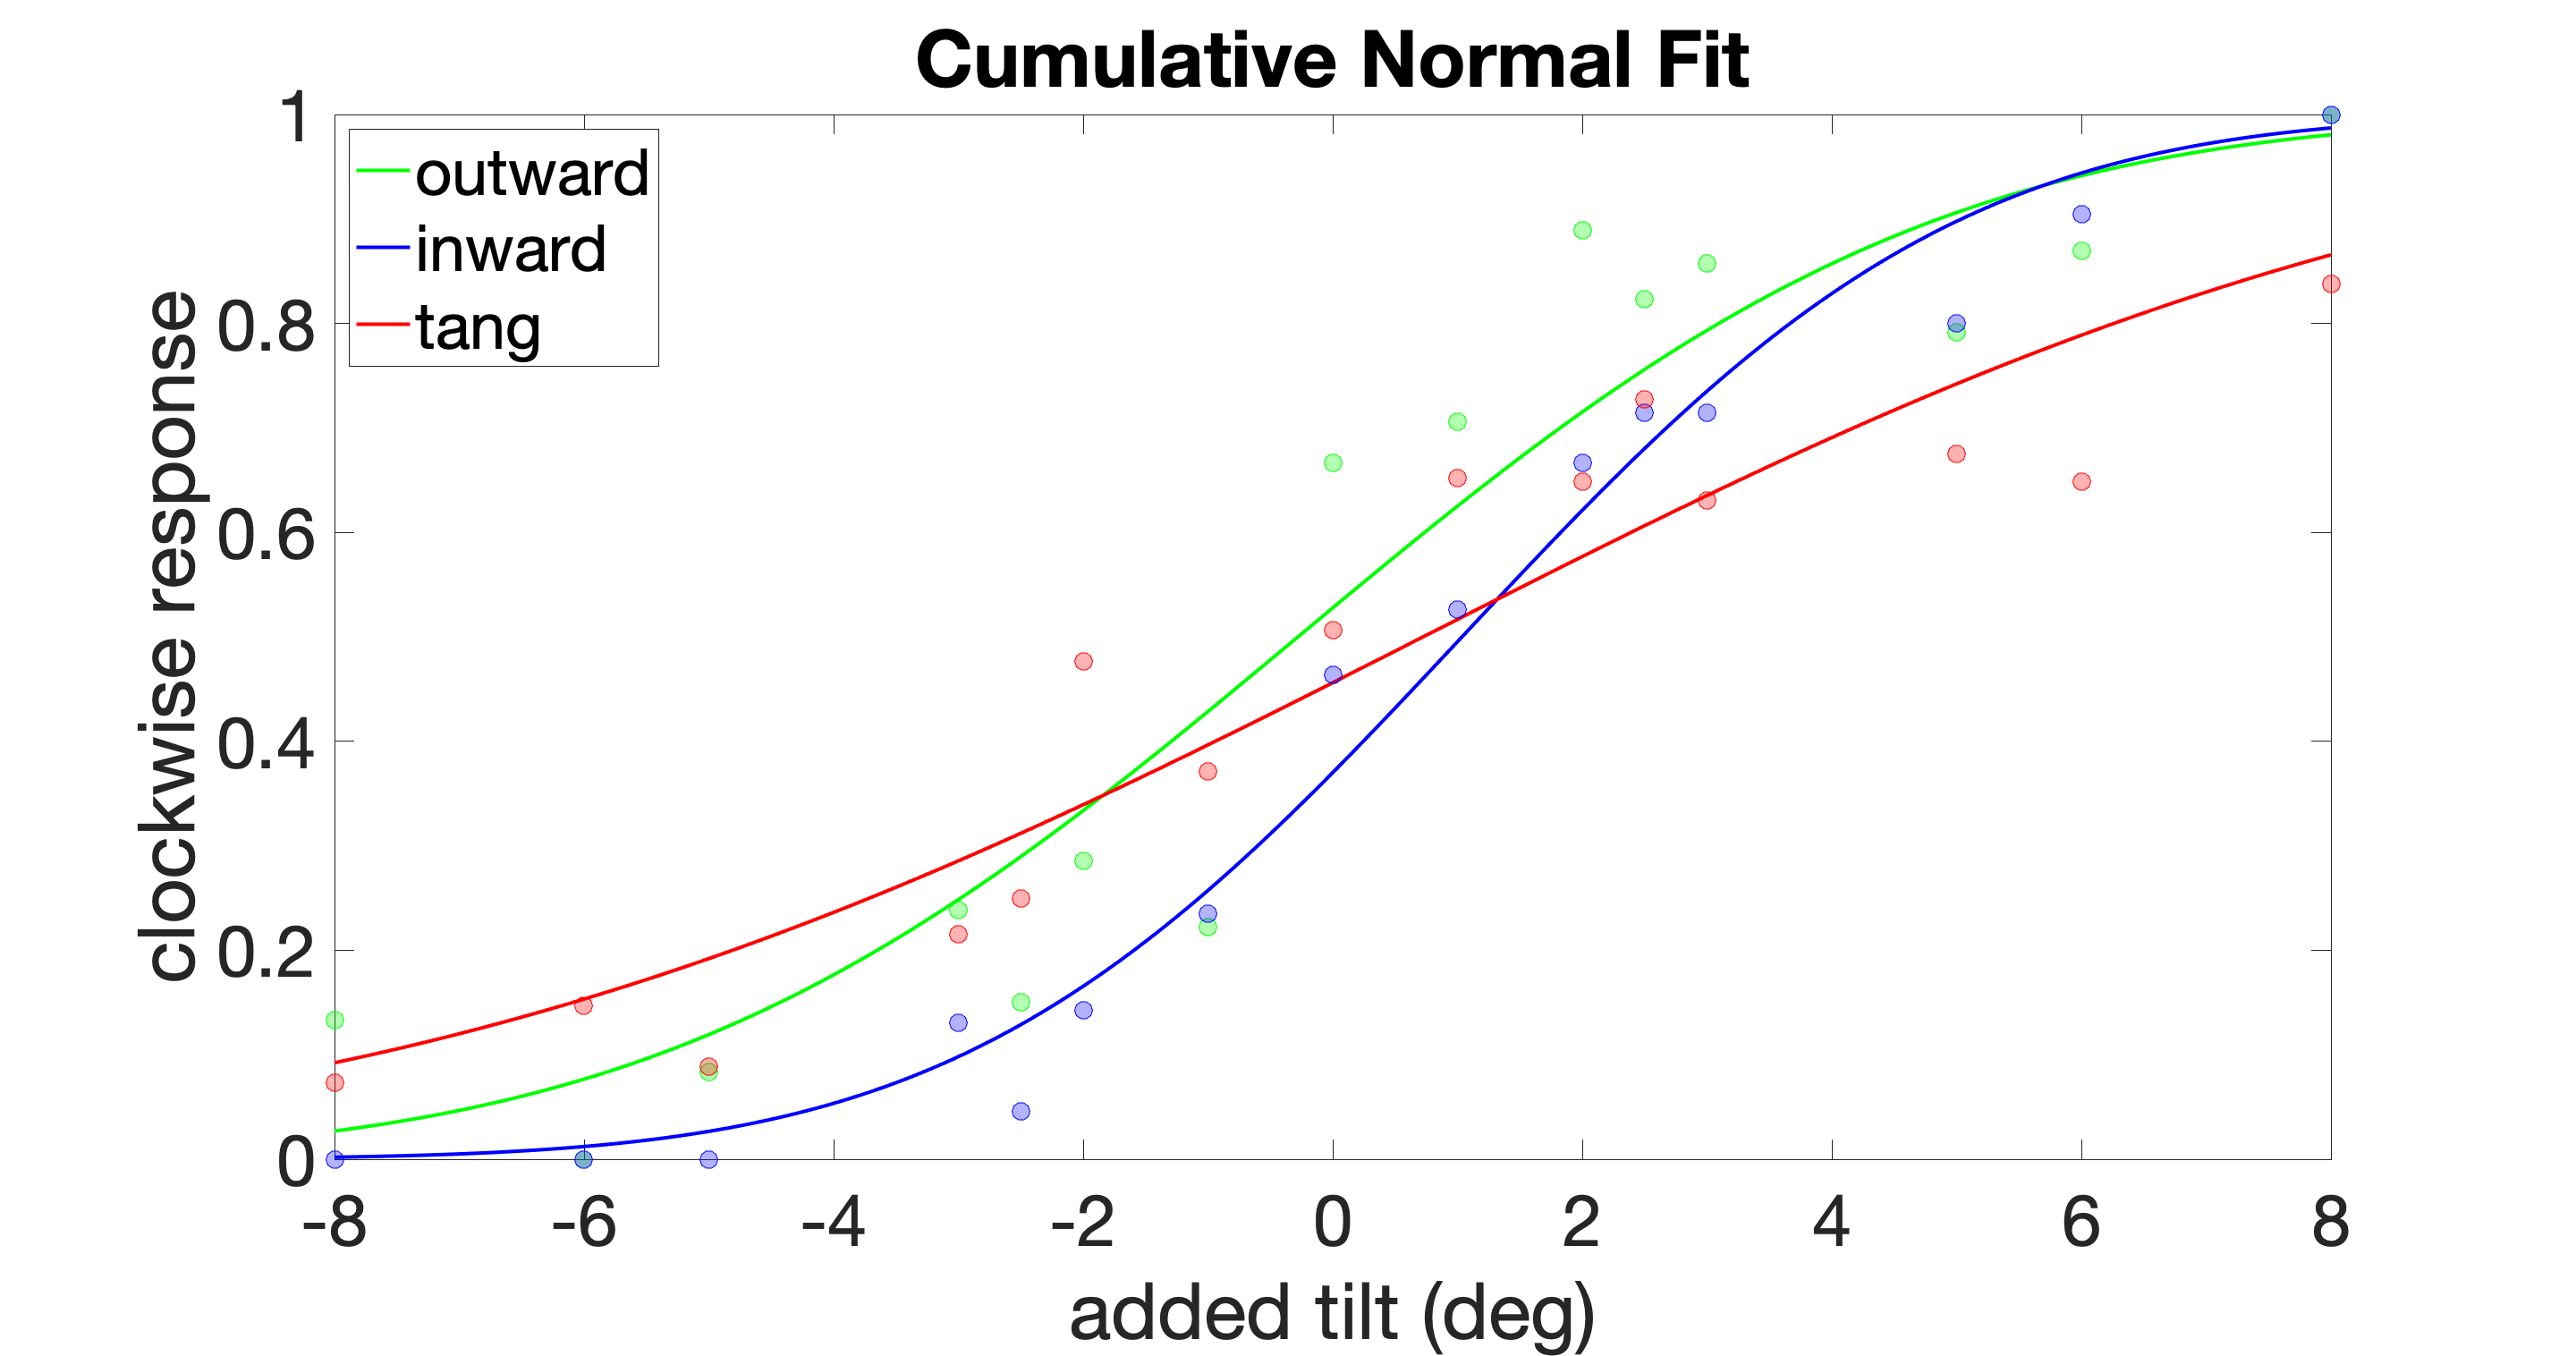
\includegraphics[scale=.08]{Images/PF_angles_old.png}
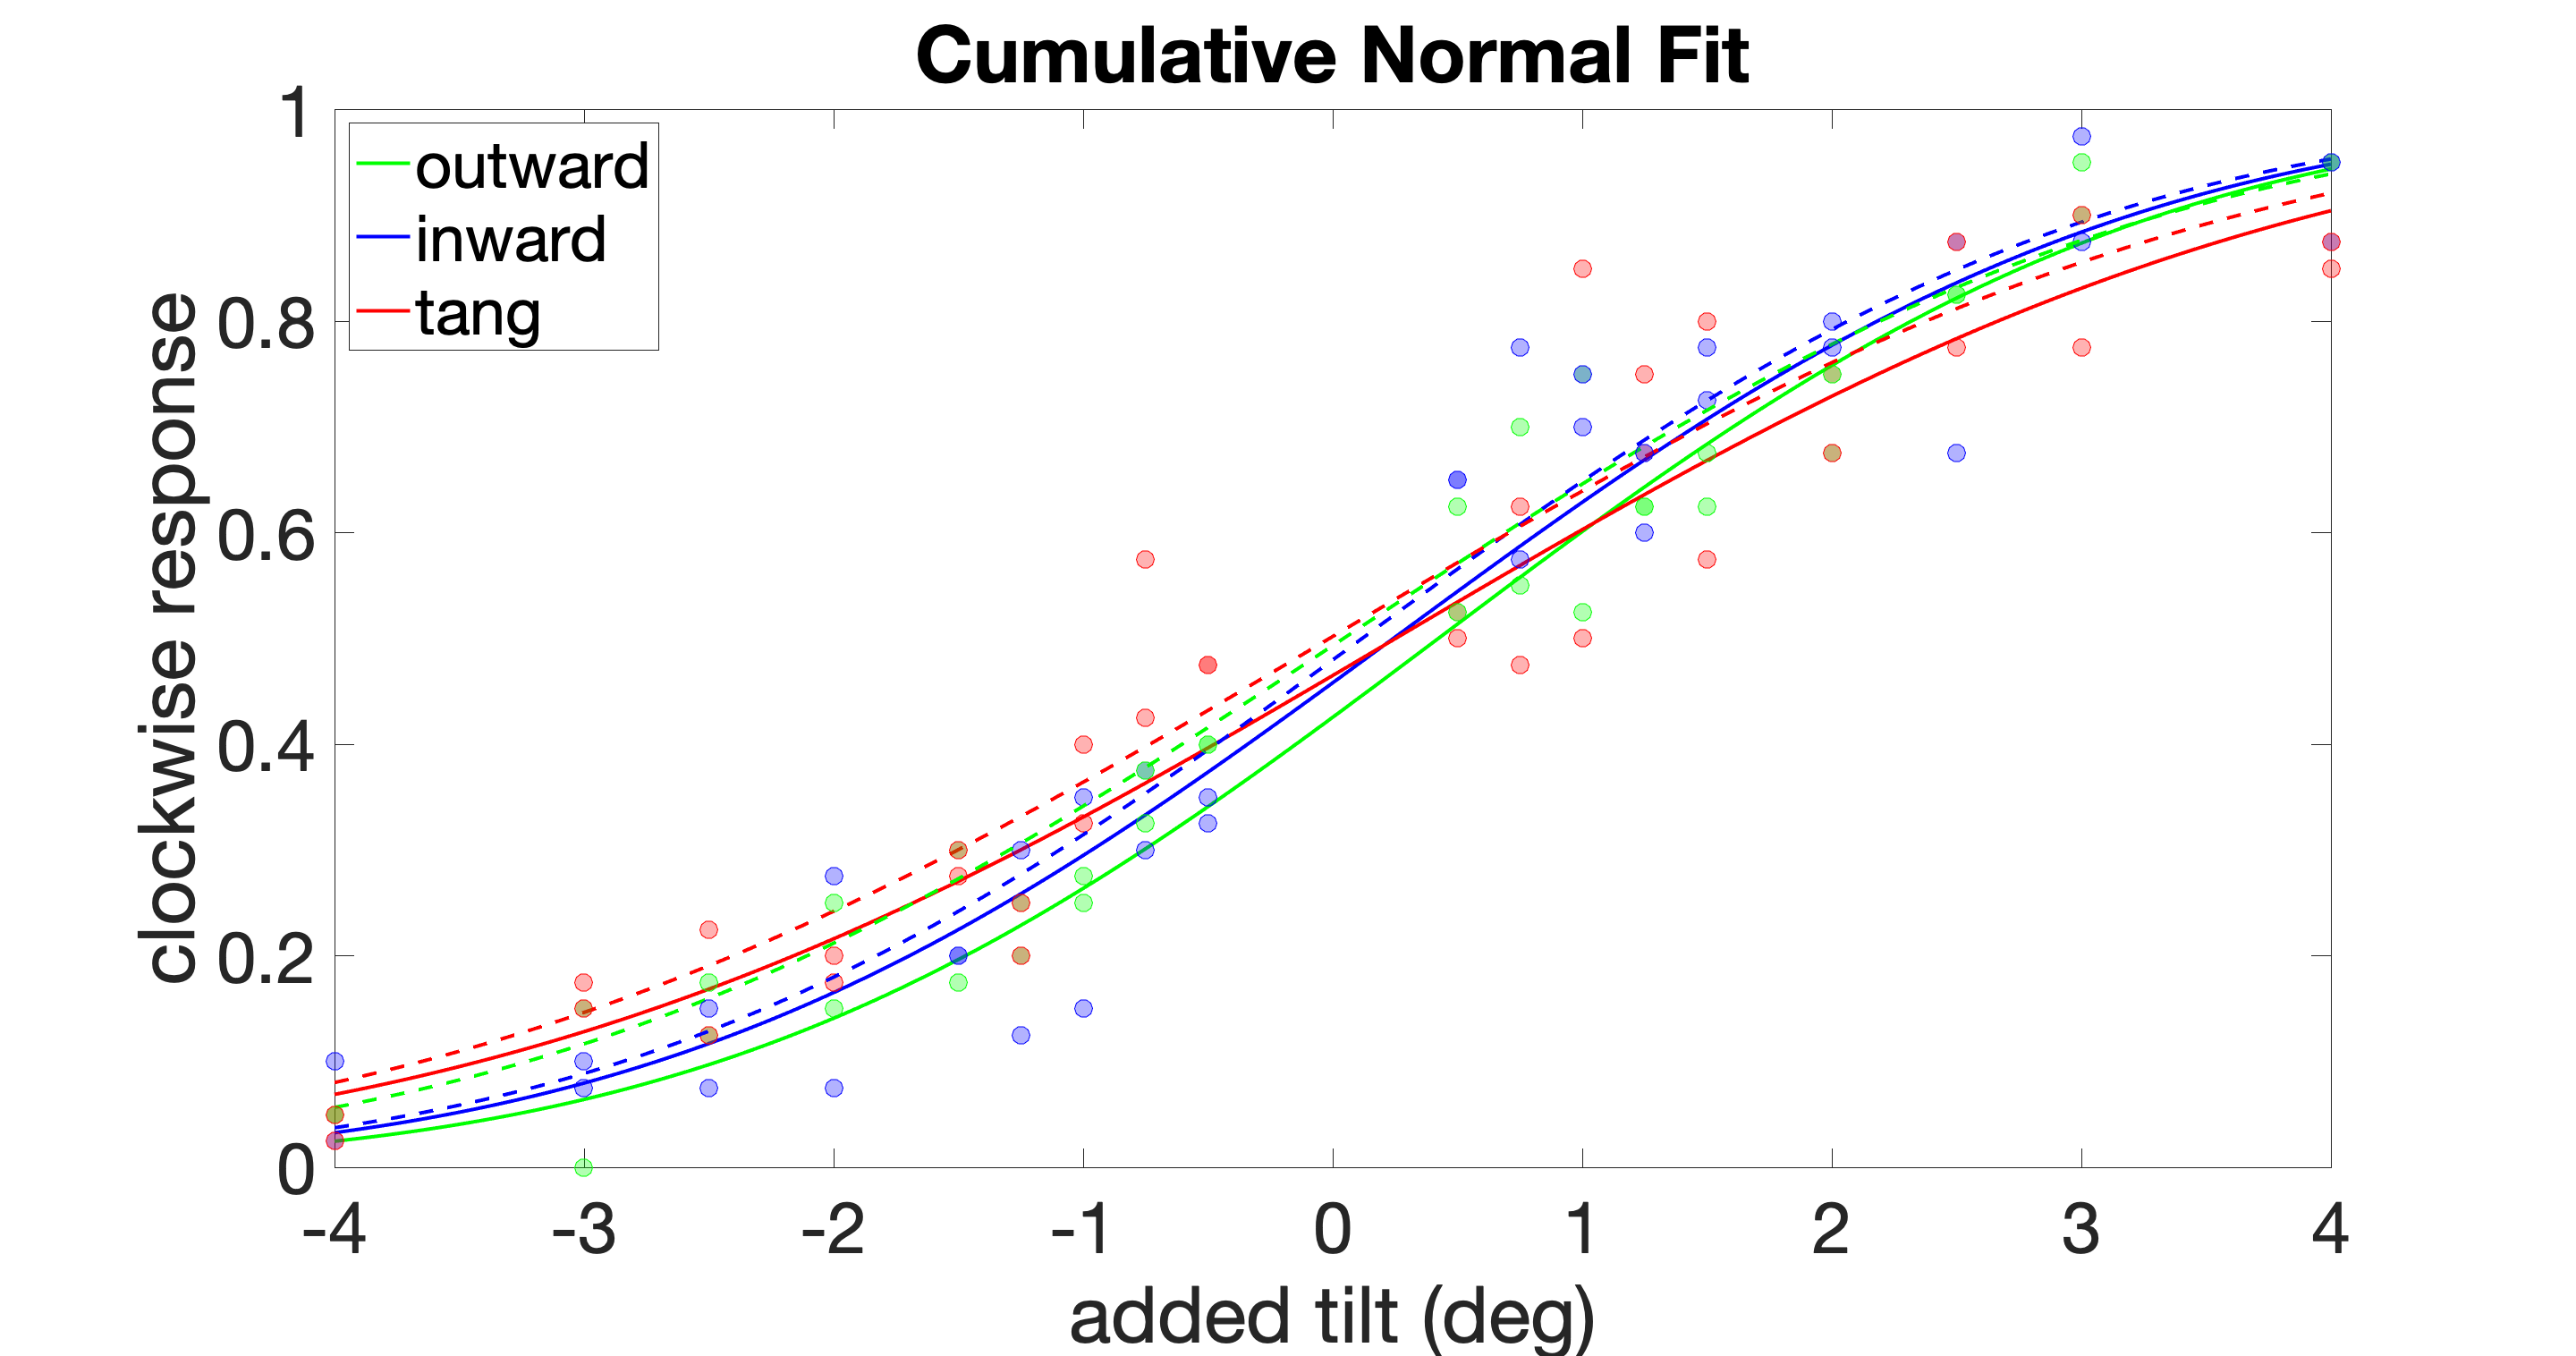
\includegraphics[scale=.08]{Images/PF_overlayed.png}
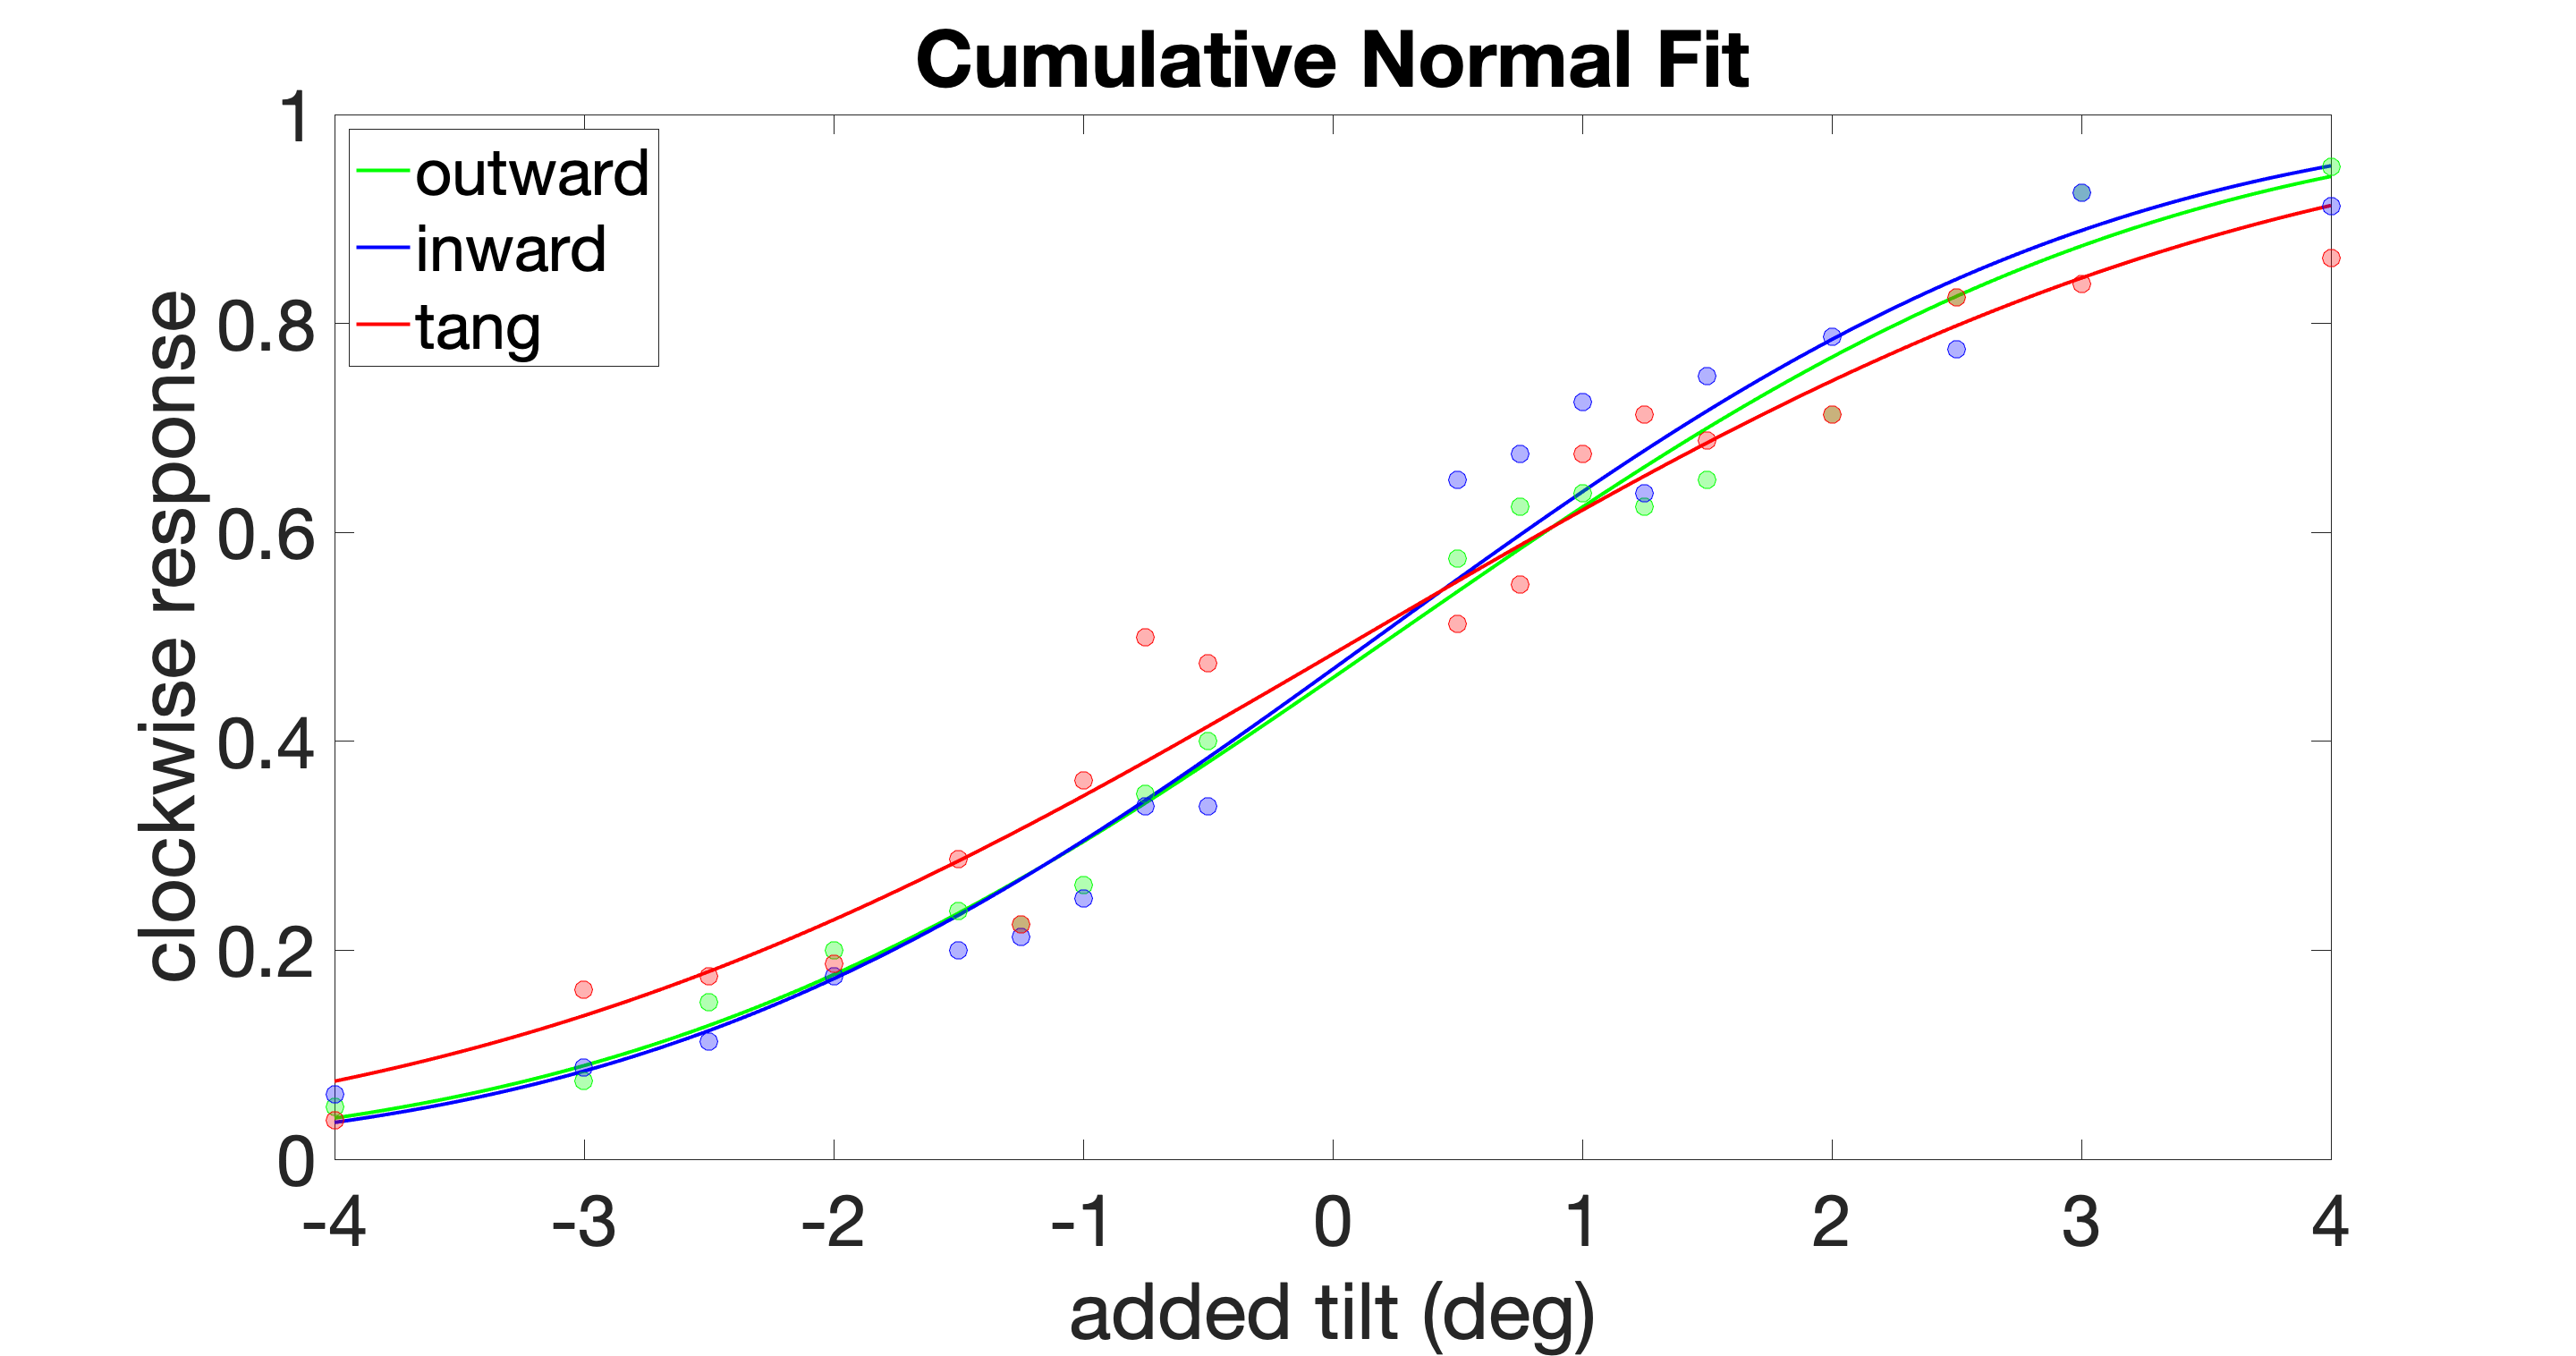
\includegraphics[scale=.08]{Images/PF_combined.png}
\caption{Top left: previous data collected with blocks separated by radial-in, radial-out, tang-c, tang-cc. Top right: new data with blocks that contain same reference vector (e.g. blocks mixing radial-in/radial-out). This combines data across locations (40 trials per angle), and shows test (solid), re-test (dotted). Bottom: new data with test and re-test combined (80 trials per angle).}
\end{figure}

\end{document}